\chapter{Polygon Geometry}
\label{ch:polygon_ops}

\section{Polygon Boolean Operations}
\label{sec:polygon_boolean}

\subsection{1. Overview}
Polygon Boolean operations are a set of geometric algorithms used to compute the result of applying set operations (union, intersection, difference, and symmetric difference) to two or more polygons~\cite{vatti1992}. These operations are essential in computer graphics, CAD/CAM, and GIS for manipulating complex shapes and defining regions of interest.

\subsection{2. Definitions}
\begin{definition}[Polygon Union]
\label{def:pb_union}
The \emph{union} $A \cup B$ of two polygons $A$ and $B$ is the region covered by at least one of the input polygons.
\end{definition}

\begin{definition}[Polygon Intersection]
\label{def:pb_intersection}
The \emph{intersection} $A \cap B$ of two polygons $A$ and $B$ is the region shared by both input polygons.
\end{definition}

\begin{definition}[Polygon Difference]
\label{def:pb_difference}
The \emph{difference} $A - B$ is the region inside polygon $A$ but outside polygon $B$.
\end{definition}

\begin{definition}[Symmetric Difference]
\label{def:pb_sym_diff}
The \emph{symmetric difference} $A \Delta B$ is the region inside either $A$ or $B$, but not both. Formally, $A \Delta B = (A - B) \cup (B - A)$.
\end{definition}

\begin{definition}[Winding Rule]
\label{def:pb_winding}
A \emph{winding rule} (e.g., Even-Odd or Non-Zero winding number) is a rule used to determine the ``inside'' of a self-intersecting or hole-containing polygon. The Even-Odd rule considers a point inside if a ray from it crosses an odd number of edges; the Non-Zero rule considers the winding number (total signed crossings).
\end{definition}

\subsection{3. Theory}
The most common approach to polygon Boolean operations is based on \textbf{edge clipping and subdivision}~\cite{greiner1998}. The algorithm typically involves:
\begin{enumerate}
    \item \textbf{Intersection Detection}: Finding all points where edges of polygon $A$ intersect edges of polygon $B$.
    \item \textbf{Edge Subdivision}: Splitting edges at intersection points into smaller segments.
    \item \textbf{Edge Classification}: For each segment, determining if it is ``Inside,'' ``Outside,'' or ``Shared'' relative to the other polygon.
    \item \textbf{Loop Assembly}: Collecting the appropriate segments based on the desired operation and assembling them into new closed loops.
\end{enumerate}

\begin{theorem}[Polygon Boolean Complexity]
\label{thm:pb_complexity}
Let $A$ and $B$ be two simple polygons with $n$ and $m$ vertices respectively, producing $k$ intersection points. The Boolean operations $A \cup B$, $A \cap B$, $A - B$, and $A \Delta B$ can all be computed in $O((n + m + k) \log(n + m))$ time using a sweep-line algorithm~\cite{vatti1992}.
\end{theorem}
\begin{proof}
The algorithm proceeds in three phases. In phase 1, we find all $k$ edge-edge intersections using a Bentley--Ottmann sweep line in $O((n+m+k)\log(n+m))$ time. In phase 2, we subdivide and classify each edge segment in $O(1)$ per segment (total $O(n+m+k)$). In phase 3, we assemble result polygons by traversing the doubly-linked edge structures in $O(n+m+k)$ time. The overall bound is dominated by the sweep.
\end{proof}

\begin{example}[Polygon Intersection Trace]
\label{ex:pb_trace}
Let $A$ be the square $[0,3] \times [0,3]$ and $B$ the square $[1,4] \times [1,4]$.
\begin{enumerate}
    \item \textbf{Intersection detection}: The edges intersect at $(1,3)$, $(3,1)$, $(1,1)$, and $(3,3)$.  Wait: $A$'s right edge $x=3$ intersects $B$'s bottom edge $y=1$ at $(3,1)$; $A$'s top edge $y=3$ intersects $B$'s left edge $x=1$ at $(1,3)$. There are $k=2$ intersection points: $(3,1)$ and $(1,3)$.
    \item \textbf{Edge subdivision}: $A$'s right edge is split into $[(3,0),(3,1)]$ and $[(3,1),(3,3)]$; $A$'s top edge is split into $[(0,3),(1,3)]$ and $[(1,3),(3,3)]$.  Similarly for $B$'s edges.
    \item \textbf{Classification}: For $A \cap B$, we keep only segments that lie inside both polygons: $[(3,1),(3,3)]$ (right edge of $A$, inside $B$), $[(1,3),(3,3)]$ (top edge of $A$, inside $B$), plus segments from $B$ inside $A$.
    \item \textbf{Assembly}: The resulting intersection is the square $[1,3] \times [1,3]$ with vertices $(1,1), (3,1), (3,3), (1,3)$.
\end{enumerate}
\end{example}

\begin{figure}[htbp]
\centering
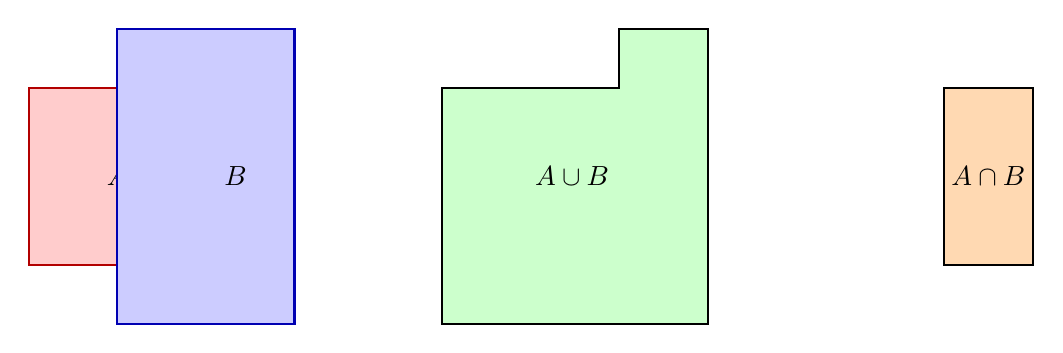
\begin{tikzpicture}[scale=0.75]
  \fill[red!20] (0,0)--(0,3)--(3,3)--(3,0)--cycle;
  \draw[thick,red!70!black] (0,0)--(0,3)--(3,3)--(3,0)--cycle;
  \node at (1.5,1.5) {$A$};
  \fill[blue!20] (1.5,-1)--(1.5,4)--(4.5,4)--(4.5,-1)--cycle;
  \draw[thick,blue!70!black] (1.5,-1)--(1.5,4)--(4.5,4)--(4.5,-1)--cycle;
  \node at (3.5,1.5) {$B$};
  \begin{scope}[xshift=7cm]
    \fill[green!20] (0,-1)--(0,3)--(3,3)--(3,4)--(4.5,4)--(4.5,-1)--cycle;
    \draw[thick] (0,-1)--(0,3)--(3,3)--(3,4)--(4.5,4)--(4.5,-1)--cycle;
    \node at (2.2,1.5) {$A \cup B$};
  \end{scope}
  \begin{scope}[xshift=14cm]
    \fill[orange!30] (1.5,0)--(1.5,3)--(3,3)--(3,0)--cycle;
    \draw[thick] (1.5,0)--(1.5,3)--(3,3)--(3,0)--cycle;
    \node at (2.25,1.5) {$A \cap B$};
  \end{scope}
\end{tikzpicture}
\caption{Polygon boolean operations: Union $A \cup B$ (center) and Intersection $A \cap B$ (right) of two overlapping rectangles.}
\label{fig:polygon_boolean}
\end{figure}


\subsection{4. Pseudo code}
\begin{algorithm}
\begin{algorithmic}[1]
\Function{PolygonBoolean}{A, B, operation}
\label{alg:polygon_boolean}
    \Comment{1. Split edges at intersection points}
    \State subdivided\_A $\gets$ SplitEdges(A, B)
    \State subdivided\_B $\gets$ SplitEdges(B, A)
    
    \Comment{2. Classify segments}
    \State classified\_A $\gets$ Classify(subdivided\_A, B)
    \State classified\_B $\gets$ Classify(subdivided\_B, A)
    
    \Comment{3. Filter segments based on operation}
    \State result\_segments $\gets$ []
    \If{operation == "UNION"}
        \State result\_segments += [s for s in classified\_A if s.is\_outside]
        \State result\_segments += [s for s in classified\_B if s.is\_outside]
    \ElsIf{operation == "INTERSECTION"}
        \State result\_segments += [s for s in classified\_A if s.is\_inside]
        \State result\_segments += [s for s in classified\_B if s.is\_inside]
    \EndIf
        
    \Comment{4. Assemble into polygons}
    \State \Return AssemblePolygons(result\_segments)
\EndFunction
\end{algorithmic}
\end{algorithm}

\subsection{5. Parameters Selections}
\begin{definition}[Precision (Epsilon)]
\label{def:pb_epsilon}
The \emph{precision} $\epsilon$ is a floating-point tolerance used to determine if a vertex lies on an edge or if two edges are collinear. It is crucial for numerical robustness.
\end{definition}

\begin{definition}[Consistent Winding]
\label{def:pb_consistent_winding}
\emph{Consistent winding} requires that both input polygons use the same orientation convention (e.g., both counter-clockwise). Most algorithms assume counter-clockwise orientation for all inputs.
\end{definition}

\subsection{6. Complexity}
\begin{theorem}[Polygon Boolean Complexity Summary]
\label{thm:pb_complexity_summary}
For two simple polygons $A$ ($n$ vertices) and $B$ ($m$ vertices) with $k$ intersection points:
\begin{enumerate}
    \item \textbf{Time}: $O((n+m+k)\log(n+m))$ using sweep-line intersection detection~\cite{vatti1992}.
    \item \textbf{Space}: $O(n+m+k)$ for the subdivided edges and output polygon.
\end{enumerate}
\end{theorem}

\subsection{7. Usages}
\begin{itemize}
    \item \textbf{CSG (Constructive Solid Geometry)}\index{CSG}: Building complex 3D objects from simple primitives.
    \item \textbf{GIS Clipping}\index{GIS clipping}: Extracting spatial data within a specific boundary (e.g., finding all roads in a county).
    \item \textbf{PCB Design}: Calculating overlapping areas of copper layers or solder masks.
    \item \textbf{UI Layout}: Determining visible regions of windows and buttons.
\end{itemize}

\subsection{8. Testing methods and Edge cases}
\begin{itemize}
    \item \textbf{Collinear Edges}: Edges that overlap exactly or partially.
    \item \textbf{Shared Vertices}: Polygons touching at a single point or along a common edge.
    \item \textbf{Holes}: Polygons containing internal voids or ``islands.''
    \item \textbf{Self-Intersecting Inputs}: May require preprocessing into a set of simple polygons.
    \item \textbf{Degeneracies}: Zero-area polygons resulting from subtraction.
\end{itemize}

\subsection{9. References}
\begin{itemize}
    \item Vatti, B. R. (1992). ``A generic solution to polygon clipping''. Communications of the ACM.
    \item Greiner, G., \& Hormann, K. (1998). ``Efficient clipping of arbitrary polygons''. ACM TOG.
    \item Weiler, K., \& Atherton, P. (1977). ``Hidden surface removal using polygon area subdivision''. SIGGRAPH.
    \item \href{https://en.wikipedia.org/wiki/Boolean_operations_on_polygons}{Wikipedia: Boolean operations on polygons}
\end{itemize}

\section{Line Arrangements}
\label{sec:line_arrangements}

\subsection{1. Overview}
A \textbf{line arrangement}\index{line arrangement} is the subdivision of the 2D plane induced by a set of $n$ lines. It is a fundamental structure in computational geometry that encodes all intersection points and the topological relationships between the lines (vertices, edges, and faces)~\cite{edelsbrunner1986}. Arrangements provide a geometric framework for solving problems involving duality, range searching, and visibility.

\subsection{2. Definitions}
\begin{definition}[Arrangement]
\label{def:la_arrangement}
Given a set $L$ of $n$ lines, the \emph{arrangement} $\mathcal{A}(L)$ is the subdivision of the plane into vertices (intersection points), edges (maximal connected portions of lines between vertices), and faces (maximal connected regions of the plane not containing any line).
\end{definition}

\begin{definition}[Zone]
\label{def:la_zone}
The \emph{zone} of a line $\ell$ in an arrangement $\mathcal{A}(L)$ is the set of faces in $\mathcal{A}(L)$ that are intersected by $\ell$.
\end{definition}

\begin{definition}[DCEL]
\label{def:la_dcel}
The \emph{Doubly-Connected Edge List (DCEL)}\index{DCEL} is the standard data structure for representing arrangements. It stores for each edge: an origin vertex, a destination vertex, a pointer to the next edge around the face, and a pointer to the twin (opposite) edge.
\end{definition}

\subsection{3. Theory}
For $n$ lines in \textbf{general position}\index{general position} (no two lines parallel, no three lines concurrent):
\begin{itemize}
    \item Number of vertices: $\binom{n}{2} = \frac{n(n-1)}{2}$.
    \item Number of edges: $n^2$.
    \item Number of faces: $\frac{n^2 + n + 2}{2}$.
\end{itemize}

The standard way to build an arrangement is through \textbf{incremental construction}:
\begin{enumerate}
    \item Start with a simple arrangement of two lines.
    \item Add lines one by one. For each new line $\ell_i$:
    \begin{itemize}
        \item Find the face containing one end of $\ell_i$.
        \item Trace the path of $\ell_i$ through the arrangement using the \textbf{Zone Theorem}.
        \item Split edges and faces as $\ell_i$ passes through them.
    \end{itemize}
\end{enumerate}

\begin{theorem}[Zone Theorem]
\label{thm:zone_theorem}
In an arrangement of $n$ lines, the zone of a single line $\ell$ has $O(n)$ complexity, i.e., it intersects $O(n)$ edges and faces~\cite{edelsbrunner1986}.
\end{theorem}
\begin{proof}
Let $\ell$ be the new line. As $\ell$ traverses the arrangement from left to right, each time it crosses an edge of the arrangement, it enters a new face. Each existing line $l_j$ intersects $\ell$ in at most one point, contributing at most 2 edges to the zone boundary (one above $\ell$, one below). Since there are $n-1$ other lines, the total zone complexity is at most $2(n-1) + 1 = O(n)$.
\end{proof}

\begin{theorem}[Arrangement Construction Complexity]
\label{thm:la_complexity}
An arrangement of $n$ lines can be constructed in $O(n^2)$ time and stored in $O(n^2)$ space using the incremental algorithm based on the Zone Theorem~\cite{edelsbrunner1986}.
\end{theorem}
\begin{proof}
We add $n$ lines one at a time. For the $i$-th line, the Zone Theorem guarantees that its zone in the arrangement of the first $i-1$ lines has $O(i)$ complexity. The cost of inserting line $i$ is therefore $O(i)$. Summing over all $n$ lines: $\sum_{i=1}^{n} O(i) = O(n^2)$.
\end{proof}

\begin{example}[Arrangement of 3 Lines]
\label{ex:la_3lines}
Consider three lines in general position: $\ell_1: y = 0$, $\ell_2: y = x$, $\ell_3: y = -x + 2$.
\begin{itemize}
    \item $\binom{3}{2} = 3$ vertices: $(0,0)$, $(1,0)$, $(1,1)$.
    \item $3^2 = 9$ edges.
    \item $\frac{9+3+2}{2} = 7$ faces: 1 bounded triangle and 6 unbounded regions.
\end{itemize}
The bounded face is the triangle with vertices $(0,0)$, $(1,0)$, and $(1,1)$.
\end{example}

\subsection{4. Pseudo code}
\begin{algorithm}
\begin{algorithmic}[1]
\Function{BuildArrangement}{lines}
\label{alg:build_arrangement}
    \Comment{1. Initialize with a large bounding box}
    \State arrangement $\gets$ InitializeDCEL()
    
    \Comment{2. Add lines incrementally}
    \For{line in lines}
        \Comment{3. Locate start face}
        \State face $\gets$ LocateFace(arrangement, line.start\_point)
        
        \Comment{4. Trace the line through the arrangement (Zone Walk)}
        \State current\_p $\gets$ line.start\_point
        \While{not IsFinished(current\_p)}
            \Comment{Find which edge of the current face the line exits through}
            \State exit\_edge $\gets$ FindExitEdge(face, line)
            
            \Comment{Split the face and update the DCEL}
            \State arrangement.SplitFace(face, line, exit\_edge)
            
            \Comment{Move to the adjacent face}
            \State face $\gets$ arrangement.GetAdjacentFace(exit\_edge)
            \State current\_p $\gets$ arrangement.GetIntersection(line, exit\_edge)
        \EndWhile
    \EndFor
    
    \State \Return arrangement
\EndFunction
\end{algorithmic}
\end{algorithm}

\subsection{5. Parameters Selections}
\begin{definition}[DCEL Representation]
\label{def:la_dcel_choice}
The \emph{Doubly-Connected Edge List (DCEL)} is the standard choice for representing arrangements as it allows for efficient traversal of vertices, edges, and faces in $O(1)$ per step.
\end{definition}

\begin{definition}[General Position Handling]
\label{def:la_general_position}
If lines can be parallel or concurrent (degenerate), the construction algorithm must use robust geometric predicates and degeneracy handling. In practice, a symbolic perturbation or an epsilon-based approach is used.
\end{definition}

\subsection{6. Complexity}
\begin{theorem}[Arrangement Complexity Summary]
\label{thm:la_complexity_summary}
For $n$ lines in general position:
\begin{enumerate}
    \item \textbf{Time}: $O(n^2)$ for construction using the incremental algorithm with the Zone Theorem.
    \item \textbf{Space}: $O(n^2)$ to store all vertices, edges, and faces.
    \item \textbf{Face Count}: $\frac{n^2+n+2}{2} = O(n^2)$.
\end{enumerate}
\end{theorem}

\subsection{7. Usages}
\begin{itemize}
    \item \textbf{Duality Problems}\index{duality}: Many problems involving points can be solved by mapping them to lines in a dual plane and analyzing their arrangement (e.g., finding the maximum number of collinear points)~\cite{chazelle1985power}.
    \item \textbf{Visibility}\index{visibility graph}: Computing the visibility graph of a set of obstacles.
    \item \textbf{Motion Planning}\index{motion planning}: Analyzing the complexity of the configuration space for a robot.
    \item \textbf{Range Searching}\index{range search}: Identifying all points within a specific region.
    \item \textbf{Statistical Analysis}: Finding the Theil-Sen estimator or other robust regression lines.
\end{itemize}

\subsection{8. Testing methods and Edge cases}
\begin{itemize}
    \item \textbf{Parallel Lines}: Verify that the algorithm correctly creates regions between lines that never intersect.
    \item \textbf{Concurrent Lines}: Ensure that three or more lines meeting at a single point are handled without creating zero-length edges.
    \item \textbf{Horizontal/Vertical Lines}: Test with lines aligned to the axes.
    \item \textbf{Small $n$}: Verify the formula for $n=1, 2, 3$.
    \item \textbf{Bounding Box}: Ensure the arrangement handles lines that extend to infinity correctly by using a sufficiently large bounding volume or symbolic coordinates.
\end{itemize}

\subsection{9. References}
\begin{itemize}
    \item Edelsbrunner, H., O'Rourke, J., \& Seidel, R. (1986). ``Constructing arrangements of lines and hyperplanes with applications''. SIAM Journal on Computing.
    \item Chazelle, B., Guibas, L. J., \& Lee, D. T. (1985). ``The power of geometric duality''. BIT Numerical Mathematics.
    \item Berg, M. de, Cheong, O., Kreveld, M. van, \& Overmars, M. (2008). ``Computational Geometry: Algorithms and Applications''. Springer-Verlag.
    \item Wikipedia: \href{https://en.wikipedia.org/wiki/Arrangement_of_lines}{Arrangement of lines}
\end{itemize}

\section{Minkowski Sums}
\label{sec:minkowski_sums}

\subsection{1. Overview}
The \textbf{Minkowski sum}\index{Minkowski sum} of two sets of points $A$ and $B$ is the set of all possible sums of a point from $A$ and a point from $B$~\cite{lozanoperez1983}. In computational geometry, this operation is primarily used with polygons (2D) or polyhedra (3D). It is a fundamental tool for motion planning, collision detection, and calculating the offset of shapes.

\subsection{2. Definitions}
\begin{definition}[Minkowski Sum]
\label{def:ms_sum}
The \emph{Minkowski sum} of two point sets $A, B \subseteq \mathbb{R}^2$ is defined as $A \oplus B = \{a + b \mid a \in A,\; b \in B\}$.
\end{definition}

\begin{definition}[Minkowski Difference]
\label{def:ms_diff}
The \emph{Minkowski difference} is $A \ominus B = \{a - b \mid a \in A,\; b \in B\} = A \oplus (-B)$. Two shapes $A$ and $B$ intersect if and only if $\mathbf{0} \in A \ominus B$.
\end{definition}

\begin{definition}[Convex Polygon Minkowski Sum]
\label{def:ms_convex}
For two \emph{convex polygons} $P$ and $Q$ with $n$ and $m$ vertices respectively, their Minkowski sum $P \oplus Q$ is also a convex polygon with at most $n + m$ vertices.
\end{definition}

\subsection{3. Theory}
For two convex polygons $P$ and $Q$ with $n$ and $m$ vertices, the Minkowski sum is computed by:
\begin{enumerate}
    \item Collect all the edges of $P$ and $Q$.
    \item Orient all edges counter-clockwise.
    \item Sort all edges by their polar angle.
    \item Chain the edges together starting from the sum of the bottom-left vertices of $P$ and $Q$.
\end{enumerate}

\begin{theorem}[Convex Minkowski Sum Complexity]
\label{thm:ms_convex}
The Minkowski sum of two convex polygons $P$ ($n$ vertices) and $Q$ ($m$ vertices) can be computed in $O(n + m)$ time and space~\cite{guibas1987}.
\end{theorem}
\begin{proof}
The edges of both polygons, when sorted by polar angle, form two sorted sequences (since both are convex). Merging two sorted sequences of total length $n+m$ takes $O(n+m)$ time. The resulting edge chain is traversed in $O(n+m)$ to form the sum polygon.
\end{proof}

For \textbf{non-convex polygons}\index{non-convex polygon}, the Minkowski sum is much more complex. The standard approach is to:
\begin{enumerate}
    \item Decompose both non-convex polygons into convex pieces (e.g., using convex decomposition).
    \item Compute the Minkowski sum for every pair of convex pieces ($P_i \oplus Q_j$).
    \item Compute the union of all the resulting convex Minkowski sums.
\end{enumerate}

\begin{theorem}[Non-Convex Minkowski Sum Complexity]
\label{thm:ms_nonconvex}
For two simple (possibly non-convex) polygons $P$ ($n$ vertices) and $Q$ ($m$ vertices), the Minkowski sum can be computed in $O(n^2 m^2)$ worst-case time.
\end{theorem}
\begin{proof}
A convex decomposition of $P$ yields at most $O(n)$ convex pieces, and similarly $O(m)$ for $Q$. Computing each pairwise sum $P_i \oplus Q_j$ takes $O(|P_i| + |Q_j|)$ time by \cref{thm:ms_convex}. The total work for $O(nm)$ pairwise sums is $O(n^2 m^2)$ in the worst case (accounting for the union step).
\end{proof}

\begin{example}[Minkowski Sum of Two Squares]
\label{ex:ms_squares}
Let $P = \{(0,0),(1,0),(1,1),(0,1)\}$ (unit square) and $Q = \{(0,0),(2,0),(2,2),(0,2\}$ ($2 \times 2$ square). Both are CCW.
\begin{enumerate}
    \item Edges of $P$: $(1,0)$, $(0,1)$, $(-1,0)$, $(0,-1)$.
    \item Edges of $Q$: $(2,0)$, $(0,2)$, $(-2,0)$, $(0,-2)$.
    \item Sorted by angle: $(1,0)$, $(2,0)$, $(0,1)$, $(0,2)$, $(-1,0)$, $(-2,0)$, $(0,-1)$, $(0,-2)$.
    \item Starting from $(0,0)+(0,0) = (0,0)$, chain the edges: $(0,0) \to (1,0) \to (3,0) \to (3,1) \to (3,3) \to (2,3) \to (0,3) \to (0,2) \to (0,0)$.
    \item Result: A $3 \times 3$ square (after merging collinear edges), with 4 vertices.
\end{enumerate}
\end{example}

\begin{figure}[htbp]
\centering
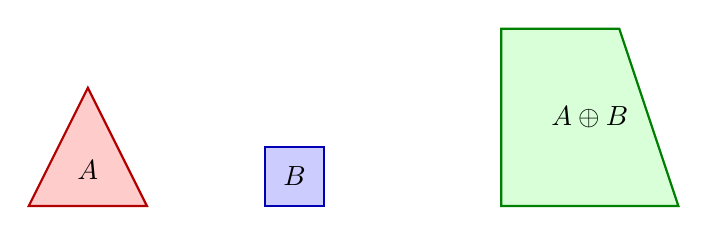
\begin{tikzpicture}[scale=0.75]
  \fill[red!20] (0,0)--(2,0)--(1,2)--cycle;
  \draw[thick,red!70!black] (0,0)--(2,0)--(1,2)--cycle;
  \node at (1,0.6) {$A$};
  \begin{scope}[xshift=4cm]
    \fill[blue!20] (0,0)--(1,0)--(1,1)--(0,1)--cycle;
    \draw[thick,blue!70!black] (0,0)--(1,0)--(1,1)--(0,1)--cycle;
    \node at (0.5,0.5) {$B$};
  \end{scope}
  \begin{scope}[xshift=8cm]
    \fill[green!15] (0,0)--(3,0)--(2,3)--(0,3)--cycle;
    \draw[thick,green!50!black] (0,0)--(3,0)--(2,3)--(0,3)--cycle;
    \node at (1.5,1.5) {$A \oplus B$};
  \end{scope}
\end{tikzpicture}
\caption{Minkowski sum of a triangle $A$ and a unit square $B$. The result is a pentagon with at most $n+m$ vertices.}
\label{fig:minkowski_sum}
\end{figure}


\subsection{4. Pseudo code}
\begin{algorithm}
\begin{algorithmic}[1]
\Function{MinkowskiSumConvex}{P, Q}
\label{alg:ms_convex}
    \Comment{P and Q are CCW convex polygons}
    \State edges\_P $\gets$ GetOrientedEdges(P)
    \State edges\_Q $\gets$ GetOrientedEdges(Q)
    
    \Comment{Sort all edges by polar angle}
    \State all\_edges $\gets$ sorted(edges\_P + edges\_Q, key=lambda e: atan2(e.dy, e.dx))
    
    \Comment{Start at the sum of bottom-left vertices}
    \State start\_P $\gets$ min(P, key=lambda p: (p.y, p.x))
    \State start\_Q $\gets$ min(Q, key=lambda p: (p.y, p.x))
    \State current $\gets$ start\_P + start\_Q
    
    \State result $\gets$ [current]
    \For{e in all\_edges}
        \State current $\gets$ current + e.vector
        \State result.append(current)
    \EndFor
        
    \State \Return result[:-1] \Comment{Remove duplicate start/end}
\EndFunction
\end{algorithmic}
\end{algorithm}

\subsection{5. Parameters Selections}
\begin{definition}[Input Orientation Requirement]
\label{def:ms_orientation}
Polygons MUST be oriented consistently (e.g., both counter-clockwise) before computing the Minkowski sum. Inconsistent orientation produces incorrect edge orderings.
\end{definition}

\begin{definition}[Convex Decomposition Method]
\label{def:ms_decomposition}
The choice of convex decomposition (exact vs.\ approximate) for non-convex inputs significantly affects the performance and quality of the non-convex Minkowski sum.
\end{definition}

\subsection{6. Complexity}
\begin{theorem}[Minkowski Sum Complexity Summary]
\label{thm:ms_complexity}
\begin{enumerate}
    \item \textbf{Convex Case}: $O(n+m)$ time and space for convex polygons $P$ ($n$ vertices) and $Q$ ($m$ vertices)~\cite{guibas1987}.
    \item \textbf{Non-Convex Case}: $O(n^2 m^2)$ worst-case time for simple polygons.
\end{enumerate}
\end{theorem}

\subsection{7. Usages}
\begin{itemize}
    \item \textbf{Motion Planning (Configuration Space)}\index{configuration space}: Expanding obstacles by the shape of the robot. If the robot's center is at $x$, it collides with obstacle $O$ if $x \in O \oplus (-\text{Robot})$~\cite{lozanoperez1983}.
    \item \textbf{Collision Detection}\index{collision detection}: The GJK (Gilbert-Johnson-Keerthi) algorithm uses Minkowski differences to check for intersections efficiently.
    \item \textbf{CAD Offsetting}: Creating a ``buffer'' or ``padding'' around a shape (mitered offsets).
    \item \textbf{Morphological Operations}\index{morphological operations}: Dilation of 2D images or 3D volumes.
\end{itemize}

\subsection{8. Testing methods and Edge cases}
\begin{itemize}
    \item \textbf{Points and Lines}: Minkowski sum of a polygon and a single point is just a translation. Sum of a polygon and a line segment is a ``swept'' version of the polygon.
    \item \textbf{Collinear Edges}: Edges from $P$ and $Q$ with the same angle should be merged into a single longer edge in the result.
    \item \textbf{Degenerate Shapes}: Polygons with zero area or zero vertices.
    \item \textbf{Non-Convex Union}: For non-convex sums, verify that internal ``voids'' are correctly handled or filled if necessary.
    \item \textbf{Origin Symmetry}: Minkowski sum of $P$ and its reflection $-P$ is always centrally symmetric.
\end{itemize}

\subsection{9. References}
\begin{itemize}
    \item Guibas, L. J., \& Seidel, R. (1987). ``Computing convolutions by reciprocal search''. Discrete \& Computational Geometry.
    \item Lozano-P\'{e}rez, T. (1983). ``Spatial Planning: A Configuration Space Approach''. IEEE Transactions on Computers.
    \item Fogel, E., \& Halperin, D. (2006). ``Exact Minkowski Sums of Convex Polygons''. CGAL Documentation.
    \item \href{https://en.wikipedia.org/wiki/Minkowski_addition}{Wikipedia: Minkowski addition}
\end{itemize}

\section{Industrial Applications of Minkowski Sums}
\label{sec:minkowski_applications}

The Minkowski sum $A \oplus B = \{a + b \mid a \in A,\, b \in B\}$
(Section~\ref{sec:minkowski_sums}) is the algebraic engine behind an
unusually broad set of industrial problems, because any operation that
``grows'' one shape by another, or that checks whether two shapes can touch,
is a Minkowski computation. The following are the principal industrial use
cases.

\begin{itemize}
\item \textbf{Robot Motion Planning (Configuration Space)}: Growing every
  obstacle by the reflected robot shape $O \oplus (-\text{Robot})$ reduces the
  moving-robot collision problem to a point-robot problem: the robot at
  translation $x$ collides iff $x \in O \oplus (-\text{Robot})$. This is the
  classical \textbf{C-space} construction of Lozano-P\'erez, and it underlies
  the collision checking of commercial offline-programming and simulation
  suites for industrial manipulators (for example, \texttt{ABB RobotStudio}
  and \texttt{FANUC Roboguide})
  (Section~\ref{sec:configuration_obstacles})~\cite{lozanoperez1983}.

\item \textbf{Collision Detection and GJK}: The Gilbert--Johnson--Keerthi
  distance algorithm computes the distance between convex shapes from a
  simplex inside the Minkowski difference $P \ominus Q$; the origin lies in
  $P \ominus Q$ exactly when the shapes intersect. GJK powers the collision
  layer of commercial physics middleware (PhysX, Havok, \texttt{Bullet}) used
  in games, film, and robotics simulation
  (Section~\ref{sec:convexint_gjk}).

\item \textbf{Assembly and Nesting (No-Fit Polygon)}: The no-fit polygon
  (NFP) used in 2D irregular cutting and packing is the Minkowski sum of one
  piece with the reflection of the other (Section~\ref{sec:hopper_optimization}
  and the definition \ref{def:nfp});
  the NFP encodes all placements where the pieces touch, driving the nesting
  engines of commercial sheet-metal, textile, and packaging software
  (SigmaNEST, Lantek, Optimation).

\item \textbf{Machine Toolpath Generation}: Offsetting a polygonal pocket by
  its tool radius via the Minkowski sum of the pocket with a disk yields the
  set of admissible tool-center positions, from which parallel or
  contour-parallel toolpaths are derived in commercial CAM systems
  (\texttt{Mastercam}, \texttt{Siemens NX CAM}, Autodesk \texttt{Fusion 360})
  for CNC machining and laser/waterjet cutting.

\item \textbf{Vehicle Swept-Path Analysis}: Computing the swept region of a
  vehicle turning along a path is a Minkowski sum of the chassis footprint
  with the path curve. It is the core of \texttt{AutoTURN} (Transoft
  Solutions), the industry-standard vehicle swept-path package used by over
  90\% of U.S. state departments of transportation for truck-turning
  clearance, bus terminals, and loading-dock design, and of the turning
  templates in the AASHTO Green Book.

\item \textbf{Autonomous Driving (Occupancy Grids)}: Inflating detected
  obstacles by the vehicle's safety margin (a Minkowski sum with a disk or
  box) builds the expanded cost map over which planners find collision-free
  paths; the same growth bounds the car's shape against lane geometry in
  commercial automated-driving stacks.

\item \textbf{Image Morphology (Dilation) in Industrial Vision}: Grayscale
  and binary dilation is the Minkowski sum of the image set with a
  structuring element, and erosion is the Minkowski difference. These are
  the workhorses of defect detection, OCR, and inspection in commercial
  machine-vision systems (Cognex, Keyence).

\item \textbf{Geometric Tolerancing (GD\&T)}: The maximum material condition
  and envelope tolerances in mechanical tolerancing are computed with
  Minkowski sums of the nominal profile with tolerance zones, bounding the
  worst-case assembled geometry in commercial tolerance-analysis packages.
\end{itemize}

\subsection{Industrial-Scale Software}
Minkowski-sum-based operations are implemented in \texttt{CGAL}
(\texttt{Minkowski\_sum\_2}, NFP and offsetting), \texttt{clipper} and
\texttt{Clipper2} (polygon offsetting; Clipper is the slicing kernel of
Ultimaker \texttt{Cura}), \texttt{Boost.Polygon} (polygon Boolean operations
and offsetting), \texttt{OMPL} (C-space construction, the planning library of
the robotics middleware \texttt{MoveIt}), and the \texttt{bullet}, PhysX, and
Havok physics engines (GJK for collision). See also the motion-planning
treatment in
Section~\ref{sec:configuration_obstacles}~\cite{lozanoperez1983,guibas1987}.

\section{Polygon Symmetry}
\label{sec:polygon_symmetry}

\subsection{1. Overview}
Polygon symmetry detection is the problem of identifying whether a given polygon possesses symmetries such as rotational symmetry or reflectional (axial) symmetry. A polygon is symmetric if it looks identical after a specific geometric transformation. Detecting these symmetries is a classic problem in computational geometry with applications in computer vision, robotics, and geometric design~\cite{atallah1985symmetry}.

\subsection{2. Definitions}
\begin{definition}[Reflectional Symmetry]
\label{def:ps_reflectional}
A polygon has \emph{reflectional (axial) symmetry} if there exists a line $\ell$ (the axis of symmetry) such that reflecting the polygon across $\ell$ maps it onto itself.
\end{definition}

\begin{definition}[Rotational Symmetry]
\label{def:ps_rotational}
A polygon has \emph{rotational symmetry} of order $k > 1$ if rotating it by $360^\circ/k$ around its centroid leaves it unchanged.
\end{definition}

\begin{definition}[Symmetry Centroid]
\label{def:ps_centroid}
The \emph{centroid} of a polygon is the average position of all the points (or vertices, for a regular polygon). For a polygon with rotational symmetry, the centroid must be the fixed point of all rotations.
\end{definition}

\subsection{3. Theory}
The most efficient algorithm for detecting polygon symmetry is based on \textbf{string matching}~\cite{atallah1985symmetry}, similar to the polygon congruence algorithm.
\begin{enumerate}
    \item Represent the polygon as a sequence of (angle, edge-length) pairs: $S = (a_1, l_1, a_2, l_2, \dots, a_n, l_n)$.
    \item \textbf{Rotational Symmetry}\index{rotational symmetry}: Find all cyclic shifts of $S$ that are identical to $S$ itself. This can be done using the \textbf{Knuth-Morris-Pratt (KMP)} algorithm by searching for $S$ in $S+S$ (excluding the trivial match at position 0).
    \item \textbf{Reflectional Symmetry}\index{reflectional symmetry}: Check if the sequence $S$ is a cyclic shift of its own reverse sequence $S^R$. If it is, the axes of symmetry must pass through either a vertex or the midpoint of an edge.
\end{enumerate}

\begin{theorem}[Polygon Symmetry Detection Complexity]
\label{thm:ps_complexity}
All rotational and reflectional symmetries of a polygon with $n$ vertices can be detected in $O(n)$ time using the string-matching approach~\cite{highnam1986}.
\end{theorem}
\begin{proof}
The signature generation takes $O(n)$ time. KMP preprocessing of the pattern $S$ takes $O(n)$, and searching $S$ in $S+S$ takes $O(n)$, giving $O(n)$ for rotational detection. Similarly, KMP on the reversed signature takes $O(n)$ for reflectional detection. The total is $O(n)$.
\end{proof}

\begin{example}[Symmetry of a Regular Hexagon]
\label{ex:ps_hexagon}
A regular hexagon has:
\begin{itemize}
    \item Rotational symmetry of order 6 ($k=6$): rotations by $0^\circ, 60^\circ, 120^\circ, 180^\circ, 240^\circ, 300^\circ$.
    \item 6 axes of reflectional symmetry: 3 passing through opposite vertices, 3 passing through midpoints of opposite edges.
\end{itemize}
The signature $S$ of a regular hexagon is $(120^\circ, s, 120^\circ, s, \dots)$ for edge length $s$. All 6 cyclic shifts of $S$ match $S$ itself, confirming order 6. The reversed signature $S^R$ matches $S$ (cyclically), confirming 6 reflection axes.
\end{example}

\subsection{4. Pseudo code}
\begin{algorithm}
\begin{algorithmic}[1]
\Function{DetectSymmetries}{polygon}
\label{alg:detect_symmetries}
    \State sig $\gets$ GenerateSignature(polygon)
    \State n $\gets$ len(polygon)
    
    \Comment{1. Detect Rotational Symmetry}
    \Comment{Find all occurrences of sig in sig + sig}
    \State rotations $\gets$ KMP\_AllMatches(sig + sig[:-1], sig)
    \State order\_k $\gets$ len(rotations)
    
    \Comment{2. Detect Reflectional Symmetry}
    \State sig\_rev $\gets$ ReverseSignature(sig)
    \State reflection\_matches $\gets$ KMP\_AllMatches(sig + sig, sig\_rev)
    
    \State axes $\gets$ []
    \For{match\_pos in reflection\_matches}
        \Comment{Calculate the axis line based on match position}
        \State axis $\gets$ CalculateAxis(match\_pos, polygon)
        \State axes.append(axis)
    \EndFor
        
    \State \Return order\_k, axes
\EndFunction

\Function{GenerateSignature}{polygon}
    \Comment{Returns (alpha\_1, d\_1, alpha\_2, l\_2, ...)}
    \Comment{where alpha is interior angle and d is edge length}
    \State \textit{pass}
\EndFunction
\end{algorithmic}
\end{algorithm}

\subsection{5. Parameters Selections}
\begin{definition}[Symmetry Precision]
\label{def:ps_precision}
Symmetry detection is highly sensitive to noise. An \emph{epsilon tolerance} should be used when comparing angles and lengths to account for floating-point imprecision.
\end{definition}

\begin{definition}[Signature Choice]
\label{def:ps_signature}
Using interior angles and edge lengths makes the detection invariant to translation, rotation, and scaling. The signature uniquely determines a polygon's shape up to congruence (or similarity if lengths are normalized).
\end{definition}

\subsection{6. Complexity}
\begin{theorem}[Polygon Symmetry Complexity Summary]
\label{thm:ps_complexity_summary}
For a polygon with $n$ vertices:
\begin{enumerate}
    \item \textbf{Signature Generation}: $O(n)$.
    \item \textbf{Rotational Check}: $O(n)$ using KMP.
    \item \textbf{Reflectional Check}: $O(n)$ using KMP on the reversed signature.
    \item \textbf{Total Time}: $O(n)$~\cite{atallah1985symmetry}.
    \item \textbf{Space}: $O(n)$ for the signature.
\end{enumerate}
\end{theorem}

\subsection{7. Usages}
\begin{itemize}
    \item \textbf{Computer Vision}\index{computer vision}: Recognizing symmetric objects (like tools, symbols, or parts) in images regardless of their orientation.
    \item \textbf{Robotics}\index{robotics}: Planning grasps for symmetric objects (where multiple orientations are equivalent).
    \item \textbf{Geometric Design (CAD)}: Enforcing symmetry constraints during modeling.
    \item \textbf{Chemistry}: Identifying the point group symmetry of molecular structures represented as polygons or polyhedra.
    \item \textbf{Art and Architecture}: Analyzing and generating symmetric patterns and tilings.
\end{itemize}

\subsection{8. Testing methods and Edge cases}
\begin{itemize}
    \item \textbf{Regular Polygons}: A regular $n$-gon should have rotational symmetry of order $n$ and $n$ axes of reflectional symmetry.
    \item \textbf{Isosceles Triangle}: Should have one axis of symmetry and no rotational symmetry ($k=1$).
    \item \textbf{Rectangle}: Should have rotational symmetry of order 2 and two axes of symmetry.
    \item \textbf{Parallelogram}: Should have rotational symmetry of order 2 but no axes of symmetry (in general).
    \item \textbf{No Symmetry}: Test on random, scalene polygons to ensure they return order 1 and zero axes.
    \item \textbf{Precision Issues}: Test with nearly symmetric polygons to verify the epsilon handling.
\end{itemize}

\subsection{9. References}
\begin{itemize}
    \item Atallah, M. J. (1985). ``On symmetry detection''. IEEE Transactions on Computers.
    \item Highnam, P. T. (1986). ``Optimal algorithms for finding the symmetries of a planar point set''. Information Processing Letters.
    \item Wolter, J. D., Woo, T. C., \& Volz, R. A. (1985). ``Optimal algorithms for detecting relevant symmetries in polygons''. IEEE Transactions on Robotics and Automation.
    \item Wikipedia: \href{https://en.wikipedia.org/wiki/Symmetry_in_geometry}{Symmetry in geometry}
\end{itemize}

\section{Polygon Matching}
\label{sec:polygon_matching}

\subsection{1. Overview}
Polygon matching is the problem of determining whether two given polygons $P$ and $Q$ are identical under a set of transformations (congruence) or whether one is a scaled version of the other (similarity)~\cite{arkin1991}. This is a specialized form of shape matching that focuses on the exact geometric properties of the boundary. It is essential for pattern recognition, computer vision, and verifying geometric designs.

\subsection{2. Definitions}
\begin{definition}[Polygon Congruence]
\label{def:pm_congruence}
Two polygons are \emph{congruent} if they have the same shape and size. They can be mapped to each other via translation, rotation, and (optionally) reflection.
\end{definition}

\begin{definition}[Polygon Similarity]
\label{def:pm_similarity}
Two polygons are \emph{similar} if they have the same shape but possibly different sizes. They can be mapped via congruence plus uniform scaling.
\end{definition}

\begin{definition}[Geometric Signature]
\label{def:pm_signature}
A \emph{geometric signature} is a sequence of values (like edge lengths and angles) that uniquely describes a polygon's shape and is invariant under certain transformations.
\end{definition}

\subsection{3. Theory}
The most robust way to check for polygon matching is to construct a \textbf{string representation} of the polygon and use string-matching algorithms~\cite{arkin1991}.
\begin{enumerate}
    \item For each vertex, calculate its \textbf{internal angle} and the \textbf{length of the edge} following it.
    \item Form a sequence: $S = (a_1, l_1, a_2, l_2, \dots, a_n, l_n)$.
    \item To handle rotation, treat the sequence as a circular string.
    \item Two polygons are congruent if their sequences are cyclic shifts of each other (or one is a cyclic shift of the reversed other, for reflection).
    \item Two polygons are similar if their angle sequences are identical and their edge length sequences are proportional.
\end{enumerate}

The \textbf{Knuth-Morris-Pratt (KMP)} algorithm can be used to find cyclic shifts in linear time by searching for sequence $S$ in $S+S$.

\begin{theorem}[Polygon Congruence via String Matching]
\label{thm:pm_congruence}
Two simple polygons $P$ and $Q$ with $n$ and $m$ vertices respectively can be tested for congruence in $O(n + m)$ time, or $O(n)$ if $n = m$~\cite{arkin1991}.
\end{theorem}
\begin{proof}
Generate the geometric signature $S_P$ for $P$ in $O(n)$ and $S_Q$ for $Q$ in $O(m)$. If $n \ne m$, reject. Otherwise, use KMP to search for $S_Q$ in $S_P + S_P$ (for rotation) and in $S_P + S_P$ for $S_Q^R$ (for reflection). Each KMP search takes $O(n)$ time.
\end{proof}

\begin{example}[Congruence Check]
\label{ex:pm_congruence}
Consider two triangles:
\begin{itemize}
    \item $P = \{(0,0),(3,0),(0,4)\}$: Edges $(3,0)$, $(-3,4)$, $(0,-4)$.  Angles: $90^\circ$ at $(0,0)$, $\arctan(4/3) \approx 53.1^\circ$ at $(3,0)$, $\arctan(3/4) \approx 36.9^\circ$ at $(0,4)$.
    \item $Q = \{(1,1),(4,1),(1,5)\}$: Same edge lengths $(3, 5, 4)$ and same angles.  Signature of $Q$ is a cyclic shift of signature of $P$.
\end{itemize}
KMP finds the match, confirming congruence.
\end{example}

\subsection{4. Pseudo code}
\begin{algorithm}
\begin{algorithmic}[1]
\Function{IsCongruent}{P, Q}
\label{alg:is_congruent}
    \If{len(P) != len(Q)}
        \State \Return False
    \EndIf
    
    \Comment{1. Generate signatures}
    \State sigP $\gets$ GenerateSignature(P)
    \State sigQ $\gets$ GenerateSignature(Q)
    
    \Comment{2. Handle reflection (optional)}
    \If{IsCyclicShift(sigP, sigQ)}
        \State \Return True
    \EndIf
    \If{IsCyclicShift(sigP, Reverse(sigQ))}
        \State \Return True
    \EndIf
    
    \State \Return False
\EndFunction

\Function{GenerateSignature}{polygon}
\label{alg:gen_signature}
    \State sig $\gets$ []
    \State n $\gets$ len(polygon)
    \For{i in range(n)}
        \State p1 $\gets$ polygon[i-1]
        \State p2 $\gets$ polygon[i]
        \State p3 $\gets$ polygon[(i+1)\%n]
        
        \State angle $\gets$ CalculateAngle(p1, p2, p3)
        \State length $\gets$ Distance(p2, p3)
        \State sig.append((angle, length))
    \EndFor
    \State \Return sig
\EndFunction

\Function{IsCyclicShift}{S1, S2}
\label{alg:is_cyclic_shift}
    \Comment{KMP search for S2 in S1 + S1}
    \State \Return KMP\_Search(S1 + S1, S2)
\EndFunction
\end{algorithmic}
\end{algorithm}

\subsection{5. Parameters Selections}
\begin{definition}[Matching Precision]
\label{def:pm_precision}
Matching should use a small epsilon for floating-point comparisons of angles and lengths. The choice of epsilon affects both false positives and false negatives.
\end{definition}

\begin{definition}[Allowed Transformations]
\label{def:pm_transformations}
Decide if reflection (mirror symmetry) is allowed. If not, only check for cyclic shifts (rotation and translation). For similarity matching, divide all edge lengths by the total perimeter or the longest edge.
\end{definition}

\subsection{6. Complexity}
\begin{theorem}[Polygon Matching Complexity Summary]
\label{thm:pm_complexity}
For two polygons with $n$ vertices each:
\begin{enumerate}
    \item \textbf{Signature Generation}: $O(n)$ each.
    \item \textbf{Matching}: $O(n)$ using KMP for cyclic shifts~\cite{arkin1991}.
    \item \textbf{Total Time}: $O(n)$ for congruence; $O(n)$ for similarity (after normalization).
    \item \textbf{Space}: $O(n)$ to store the signatures.
\end{enumerate}
\end{theorem}

\subsection{7. Usages}
\begin{itemize}
    \item \textbf{Computer Vision}\index{computer vision}: Identifying an object in an image by matching its contour to a template.
    \item \textbf{CAD/CAM}: Finding duplicate parts in a complex mechanical assembly.
    \item \textbf{Architecture}: Identifying repeating patterns or tiles in a floor plan.
    \item \textbf{Geographic Information Systems (GIS)}\index{GIS}: Matching building footprints across different map revisions.
    \item \textbf{Character Recognition}\index{character recognition}: Matching the strokes of a drawn letter to a font database.
\end{itemize}

\subsection{8. Testing methods and Edge cases}
\begin{itemize}
    \item \textbf{Rotated Polygons}: Verify that a polygon matches its rotated version.
    \item \textbf{Mirrored Polygons}: Test if the algorithm correctly identifies reflections.
    \item \textbf{Regular Polygons}: A regular $n$-gon should have $n$ different valid cyclic shifts.
    \item \textbf{Degenerate Polygons}: Test on triangles or polygons with collinear vertices.
    \item \textbf{Self-Intersecting Polygons}: Ensure the signature is robust for non-simple polygons.
    \item \textbf{Numerical Sensitivity}: Test with polygons having very small edges or angles.
\end{itemize}

\subsection{9. References}
\begin{itemize}
    \item Arkin, E. M., Chew, L. P., Huttenlocher, D. P., Kedem, K., \& Mitchell, J. S. (1991). ``An efficiently computable metric for comparing polygonal shapes''. IEEE Transactions on Pattern Analysis and Machine Intelligence.
    \item Manber, U. (1989). ``Introduction to Algorithms: A Creative Approach''. Addison-Wesley.
    \item Wikipedia: \href{https://en.wikipedia.org/wiki/Congruence_(geometry)}{Congruence (geometry)}
\end{itemize}

\section{Line and Polygon Clipping}
\label{sec:polygon_clipping}

\subsection{1. Overview}
\index{clipping}Clipping removes the portions of geometric objects lying outside a given window. Line clipping restricts a line segment to a convex window, and polygon clipping restricts a polygon to a convex window, yielding a new polygon. These operations are central to graphics viewport clipping and to Boolean operations on polygons~\cite{sutherland1974,cyrus1978}.

\subsection{2. Definitions}

\begin{definition}[Clip Window]\label{def:clip_window}
A \emph{clip window} is a (usually convex) region against which an object is clipped; the result is the intersection of the object with the window.
\end{definition}

\begin{definition}[Cyrus--Beck Clipping]\label{def:cyrus_beck}
The \emph{Cyrus--Beck} algorithm clips a line segment to a convex polygon by computing, for each boundary edge, the interval of parameters $t \in [0,1]$ for which the segment lies on the inner side, and intersecting these intervals~\cite{cyrus1978}.
\end{definition}

\begin{definition}[Sutherland--Hodgman Clipping]\label{def:sutherland_hodgman}
The \emph{Sutherland--Hodgman} algorithm clips a polygon to a convex window by successively clipping the polygon against each boundary edge of the window, producing an output polygon at every stage~\cite{sutherland1974}.
\end{definition}

\subsection{3. Theory}
Cyrus--Beck expresses the segment as $p(t) = p_0 + t(p_1 - p_0)$ and, for each window edge with inward normal $n_i$ through point $q_i$, keeps parameters satisfying $n_i \cdot (p(t) - q_i) \ge 0$. Intersecting all such $t$-intervals yields the clipped segment. Sutherland--Hodgman clips the vertex list once per window edge, retaining vertices on the inside and inserting intersection points where an edge crosses the clipping line.

\subsection{4. Pseudo code}
\begin{algorithmic}
\Function{ClipPolygon}{$P$, window $W$}
    \State $output \gets P$
    \For{each boundary edge $e$ of $W$}
        \State $input \gets output,\; output \gets \emptyset$
        \For{each edge $(s, p)$ of $input$}
            \If{$p$ inside $e$}
                \If{$s$ not inside $e$}
                    \State output $\leftarrow$ intersection of $(s,p)$ with $e$
                \EndIf
                \State output $\leftarrow p$
            \ElsIf{$s$ inside $e$}
                \State output $\leftarrow$ intersection of $(s,p)$ with $e$
            \EndIf
        \EndFor
    \EndFor
    \State \Return $output$
\EndFunction
\end{algorithmic}

\subsection{5. Parameters Selections}
\begin{itemize}
    \item \textbf{Window convexity}: Sutherland--Hodgman assumes a convex window; for non-convex windows the polygon is first decomposed or the operation handled by general Boolean intersection.
    \item \textbf{Tolerance}: use a small epsilon when classifying vertices as inside or on the boundary.
\end{itemize}

\subsection{6. Complexity}
Cyrus--Beck clips a segment against an $m$-edge convex window in $O(m)$ time. Sutherland--Hodgman clips an $n$-vertex polygon against an $m$-edge window in $O(nm)$ time.

\subsection{7. Usages}
\begin{itemize}
    \item \textbf{Graphics}: viewport and scissor clipping in the rendering pipeline.
    \item \textbf{CAD and GIS}: windowing queries and map clipping to regions of interest.
    \item \textbf{Boolean operations}: clipping is the primitive behind polygon intersection~\cite{vatti1992}.
\end{itemize}

\subsection{8. Testing methods and Edge cases}
\begin{itemize}
    \item \textbf{Window fully inside}: the polygon is returned unchanged.
    \item \textbf{Polygon fully outside}: an empty polygon is returned.
    \item \textbf{Vertex on boundary}: verify the on-edge case is not counted twice.
    \item \textbf{Degenerate output}: clipping to a triangle or segment must not produce repeated vertices.
\end{itemize}

\subsection{9. References}
\begin{itemize}
    \item Sutherland, I. E., \& Hodgman, G. W. (1974). ``Reentrant polygon clipping''. Communications of the ACM.
    \item Cyrus, M., \& Beck, J. (1978). ``Generalized two- and three-dimensional clipping''. Computers \& Graphics.
    \item Wikipedia: \href{https://en.wikipedia.org/wiki/Sutherland%E2%80%93Hodgman_algorithm}{Sutherland--Hodgman algorithm}
\end{itemize}
